\chapter{Disc samples}
\label{ch:disc}

\section{The idea}

Many flat samples are not rectangular but round: a flat circular cell (window, liquid, window), a pressed pellet, a powder held
between two circular windows, a single-crystal wafer. Version~2.3 adds this geometry: a \textbf{disc} (circular plate) made of
layers stacked along its normal, like a pile of coins of different materials (Figure~\ref{fig:disc}).

\begin{itemize}
  \item Every layer is a disc of the \textbf{same diameter} $D$ (radius $R=D/2$) and of its own thickness.
  \item The centre of the disc is on the \textbf{beam axis}: the disc goes from $y=-R$ to $y=+R$ and from $x=-R$ to $x=+R$.
  \item By default the plane of the disc is \textbf{perpendicular} to the beam. It can be \textbf{rotated} around the vertical axis
        exactly as the slab, with the plane angle $\alpha$ (\code{plane_angle_deg}, Chapter~\ref{ch:geometry}).
  \item A layer has the \textbf{same properties} as in the slab and in the cylinder: label, thickness, $\mu$, scatter fraction and the
        vertical extent of its material (\code{bottom} and \code{height}, Chapter~\ref{ch:partial}). A round cell half filled with a
        liquid is described exactly as a rectangular one.
\end{itemize}
The disc is, in fact, a slab whose section is a circle instead of a rectangle. Everything that does not depend on the shape of the
section (layers along the normal, rotation, frames, partial filling, interaction points, multiple scattering, direct method) is
shared with the slab, and all the analysis modules work with it without any change.

\begin{figure}[H]
  \centering
  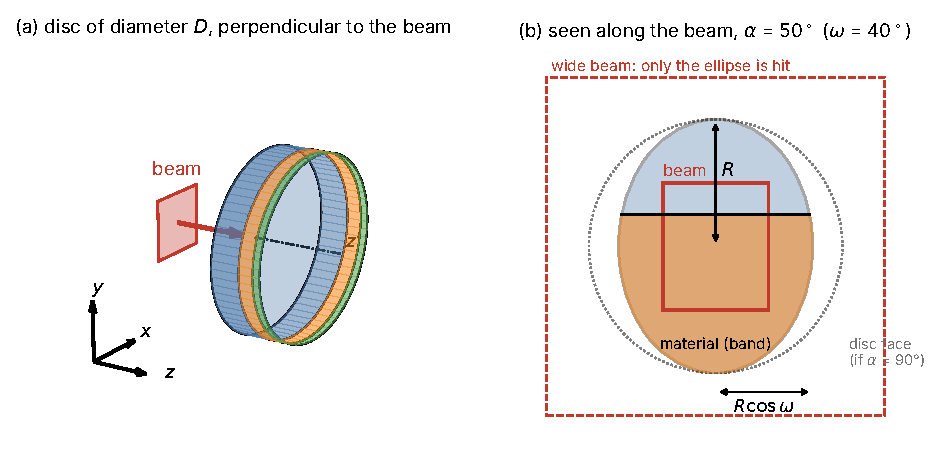
\includegraphics[width=\textwidth]{fig_disc_geometry}
  \caption{Disc geometry. (a)~Three-layer disc perpendicular to the beam; $z'$ is its normal, through the centre of the
  disc and of the beam. (b)~The disc seen along the beam when its plane makes the angle $\alpha=50^\circ$ with the beam: the face
  looks like an ellipse with vertical semi-axis $R$ and horizontal semi-axis $R\cos\omega$, $\omega=90^\circ-\alpha$. A beam
  smaller than the ellipse (solid rectangle) hits the disc everywhere; of a wide beam (dashed) only the part inside the ellipse
  meets the sample. The shaded band is the material of a partially filled layer.}
  \label{fig:disc}
\end{figure}

\section{Geometry and conventions}

The disc uses the sample frame of the slab: $z'$ is the normal of the layers, $x'$ (horizontal) and $y'=y$ (vertical) lie in their
plane, and the front face is at $z'=z_\mathrm{front}$ (default 0). Layer $i$ occupies
\begin{equation}
  x'^2 + y'^2 \le R^2, \qquad z'_i \le z' \le z'_{i+1}, \qquad b_i \le y' \le t_i,
  \label{eq:disc-layer}
\end{equation}
where $z'_i$ are the boundaries of the layers (cumulated thicknesses from the front face) and $b_i$, $t_i$ the bottom and top of
its material (by default the whole disc, $-R$ to $+R$).

\begin{description}
  \item[Rotation.] As for the slab: for $\alpha<90^\circ$ the normal is tilted towards $+x$ by $\omega=90^\circ-\alpha$; for
        $\alpha>90^\circ$ towards $-x$. The axis of rotation is the vertical line through the centre of the front face, which is on the
        beam axis. Seen along the beam the face is an ellipse of semi-axes $R\cos\omega$ (horizontal) and $R$ (vertical).
  \item[Vertical extent.] The sample height is fixed by the disc: $y_\mathrm{bottom}=-R$, $y_\mathrm{top}=+R$. The bands of the layers
        are cut at the rim. In the forms of version~2.0, \code{fill_height} is measured from the lowest point of the disc ($y=-R$) and
        \code{fullness} from the bottom of the beam, as for the other geometries.
  \item[Fullness.] \code{beam_fullness()} is, as always, the fraction of the beam \emph{height} covered by the band of the material
        (eq.~\ref{eq:fullness-general}). For a disc this is also the fraction of the interacting particles only when the beam is
        inside the disc; when the beam is wider than the chord of the disc at some heights, the illuminated width depends on $y$.
\end{description}

\begin{note}[The disc compared with the slab and the cylinder]
For a beam that stays inside the disc and directions that leave through the front or back face, a disc and a slab with the
same layers give \emph{identical} results: the section does not matter. The disc differs from the slab when particles reach its
edge: a beam wider than the disc, scattering nearly parallel to its plane ($\twotheta$ close to $\alpha \pm 90^\circ$, and close to
$90^\circ$ at normal incidence), and multiple scattering, which travels far in the plane. The disc is not a short cylinder: in a
cylinder of \mcams\ the layers are concentric shells around a vertical axis, in a disc they are stacked along a horizontal normal.
\end{note}

\section{Creating a disc sample}

\begin{fnbox}{create\_disc\_sample(diameter, layers, z\_front=0.0, plane\_angle\_deg=90.0, beam\_height=None)}
\code{diameter}: diameter of the disc (mm), the same for all the layers.
\code{layers}: from the front face to the back; tuples, dictionaries or \code{Layer} objects, as for the slab.
\code{z_front}: position of the front face along the normal (mm).
\code{plane_angle_deg}: angle between the beam and the plane of the disc, $0<\alpha<180^\circ$; 90 = perpendicular (default).
\code{beam_height}: height of the beam (mm), needed for \code{fullness} and \code{beam_fullness()}.
Returns a \code{DiscSample}.
\end{fnbox}

\begin{lstlisting}
from toscana.corrections.mcams.disc import create_disc_sample
from toscana.corrections.mcams.sample_base import Layer

cell = create_disc_sample(20.0, [("V",  0.2, 0.046, 0.78),        # front window
                                 ("Ni", 2.0, 0.180, 0.94),        # powder
                                 ("V",  0.2, 0.046, 0.78)])       # back window
tilted = create_disc_sample(20.0, [("V", 0.2, 0.046, 0.78), ("Ni", 2.0, 0.18, 0.94),
                                   ("V", 0.2, 0.046, 0.78)], plane_angle_deg=45)
half = create_disc_sample(20.0, [("V", 0.2, 0.046, 0.78),
                                 Layer("Ni", 2.0, 0.18, 0.94, bottom=-10.0, height=11.0),
                                 ("V", 0.2, 0.046, 0.78)], beam_height=8.0)
\end{lstlisting}
With the factory (Chapter~\ref{ch:sample}) the geometry is \code{"disc"} and the diameter is required; \code{height},
\code{width} and \code{y_bottom} are not used, because the disc is centred on the beam:
\begin{lstlisting}
from toscana.corrections.mcams.sample_factory import make_sample
sample = make_sample("disc", layers, diameter=20.0, plane_angle_deg=60, beam_height=8.0)
\end{lstlisting}
The names \code{"disk"}, \code{"circular"}, \code{"circular plate"} and \code{"round plate"} are accepted as well.

\section{What the disc sample tells you}

A \code{DiscSample} has all the attributes and methods of the slab (Table~\ref{tab:interface} and Chapter~\ref{ch:partial}) and a
few of its own:
\begin{center}\small
\begin{tabular}{@{}>{\raggedright\arraybackslash}p{5.6cm}p{9.2cm}@{}}
  \toprule \textbf{Attribute or method} & \textbf{Content} \\ \midrule
  \code{sample.diameter}, \code{sample.radius} & $D$ and $R$ (mm) \\
  \code{sample.summary()} & table of the layers, with the band of each one and its fullness \\
  \code{sample.face_area_in_beam(w_b, h_b)} & area (mm$^2$) of the part of a uniform $w_b\times h_b$ beam that hits the front face, seen along the beam (ellipse of semi-axes $R\cos\omega$ and $R$); exact for a thin disc. Divided by $w_b h_b$ it is the fraction of the beam that meets the sample. \\
  \code{sample.with_plane_angle(a)} & a copy of the disc with another orientation \\
  \code{sample.boundaries}, \code{z_front}, \code{z_back}, \code{total_thickness} & positions of the layers along the normal (mm), as for the slab \\
  \code{sample.width}, \code{sample.height} & both equal to $D$: the square that contains the disc (used, for instance, to place the start of the particles) \\
  \code{sample.contains(p)} & True for points with $x'^2+y'^2\le R^2$ between the two faces \\ \bottomrule
\end{tabular}
\end{center}
The area of the face seen along the beam is
\begin{equation}
  S = \int_{|y| < \min(R,\,h_b/2)} \min\!\left(2R\cos\omega\,\sqrt{1-y^2/R^2},\; w_b\right) \deriv{y},
\end{equation}
computed by the trapezoidal rule on a fine grid; for a beam larger than the ellipse at normal incidence it is $\pi R^2$.

\section{Example}

\pyexample{ex11_disc}

The beam of $8\times8$~mm is inside the disc, so the fraction of particles that interact in the Ni is the Beer--Lambert value for a
plate, $\e^{-\mu_V t_V}(1-\e^{-\mu_\mathrm{Ni} t_\mathrm{Ni}})$. The transmission is lowest at $90^\circ$, where the scattered particles
travel in the plane of the disc towards its rim. Rotating the disc to $45^\circ$ lengthens the path of the beam in the sample
($1/\sin\alpha$) and more particles interact. With a beam of $30\times30$~mm only the part that hits the face can interact: 35\% of
the beam at normal incidence ($\pi R^2/900$), 25\% at $45^\circ$, where the disc looks narrower. The partially filled disc has Ni up
to $y=+1$~mm, i.e.\ 5 of the 8~mm of the beam (fullness 0.625).

\section{How it is computed}
\label{sec:disc-algorithm}

The slab finds, for every layer, the interval $[s_0^{(i)},s_1^{(i)}]$ of a straight path $\vec p + s\,\hat d$ that lies in its
material, as the intersection of three intervals: the box of the sample, the slice of the layer and the band of the material
(Section~\ref{sec:partial-algorithm}). The disc replaces only the first of them, the \emph{section}: the box is replaced by the
cylinder $x'^2+y'^2\le R^2$ (axis along the normal $z'$) between the front and back faces.

A cylinder is convex, so a straight line is inside it during \emph{one} interval. The line meets its surface when
\begin{equation}
  (p_x + s\,d_x)^2 + (p_y + s\,d_y)^2 = R^2
  \quad\Longleftrightarrow\quad
  a\,s^2 + 2b\,s + c = 0,
\end{equation}
with $a=d_x^2+d_y^2$, $b=p_xd_x+p_yd_y$, $c=p_x^2+p_y^2-R^2$ (sample frame, primes omitted). The two roots
\begin{equation}
  s_\pm = \frac{-b \pm \sqrt{b^2 - a\,c}}{a}
\end{equation}
are where the line enters and leaves the cylinder. If $b^2-ac<0$ the line misses it. If $a=0$ the particle moves along the normal:
it is inside for ever if $c\le0$ and never otherwise. Intersected with the interval between the two faces (the same function as
for the slab), this gives the part of the path inside the disc. From then on the calculation is the slab's: the intervals of
the layers are sorted along the path, their optical depths are accumulated, and the next interaction is found where the
cumulated optical depth reaches the random value $\tau=-\ln(1-u)$ (Chapter~\ref{ch:physics}).

In the code this is a single method. \code{SlabSample} computes the section in \code{_section_interval}, and \code{DiscSample},
a subclass of \code{SlabSample}, redefines it:
\begin{lstlisting}
class DiscSample(SlabSample):
    def _section_interval(self, p, d):
        c_lo, c_hi = _cylinder_interval(p[:, 0], p[:, 1], d[:, 0], d[:, 1], self.radius)
        z_lo, z_hi = _slice_interval(p[:, 2], d[:, 2], self.z_front, self.z_back)
        return np.maximum(c_lo, z_lo), np.minimum(c_hi, z_hi)
\end{lstlisting}
It also redefines \code{contains} (inside the cylinder and between the faces), \code{_clip_inside} (a point that rounding errors
put a few $10^{-15}$~mm outside the rim is moved radially back onto it), \code{summary} and \code{with_plane_angle}, and adds
\code{face_area_in_beam}. Everything else is inherited. The slab itself was only reorganised (the box test moved into
\code{_section_interval}); its results are bit-for-bit those of version~2.2 (Chapter~\ref{ch:validation}).

\section{Results}
\label{sec:disc-results}

The figures of this section use the example layers of the main script (\code{DISC_LAYERS}: Al 2~mm, Fe 1~mm, Cu 0.5~mm, the same as
the example slab), a disc of 20~mm and a beam of $8\times8$~mm.

\begin{figure}[H]
  \centering
  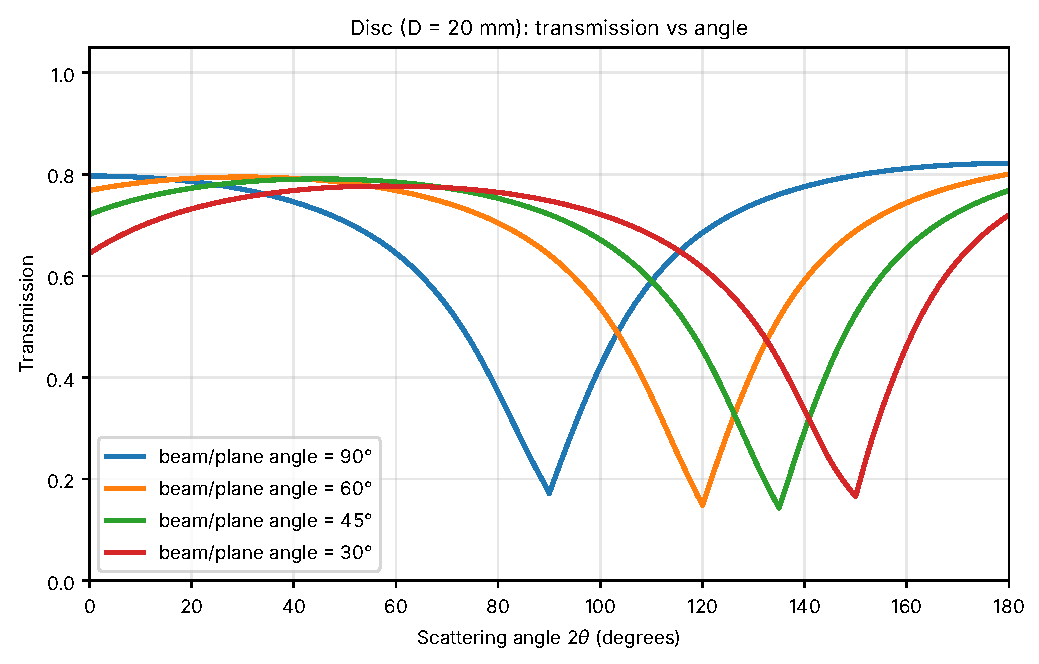
\includegraphics[width=0.78\textwidth]{fig_transmission_disc}
  \caption{Example disc: transmission of the singly scattered particles versus $\twotheta$, for four orientations. The minimum is
  where the scattered particles travel in the plane of the disc, at $\twotheta = 180^\circ-\alpha$ (detector on the side towards which
  the normal is tilted).}
  \label{fig:transdisc}
\end{figure}

\begin{figure}[H]
  \centering
  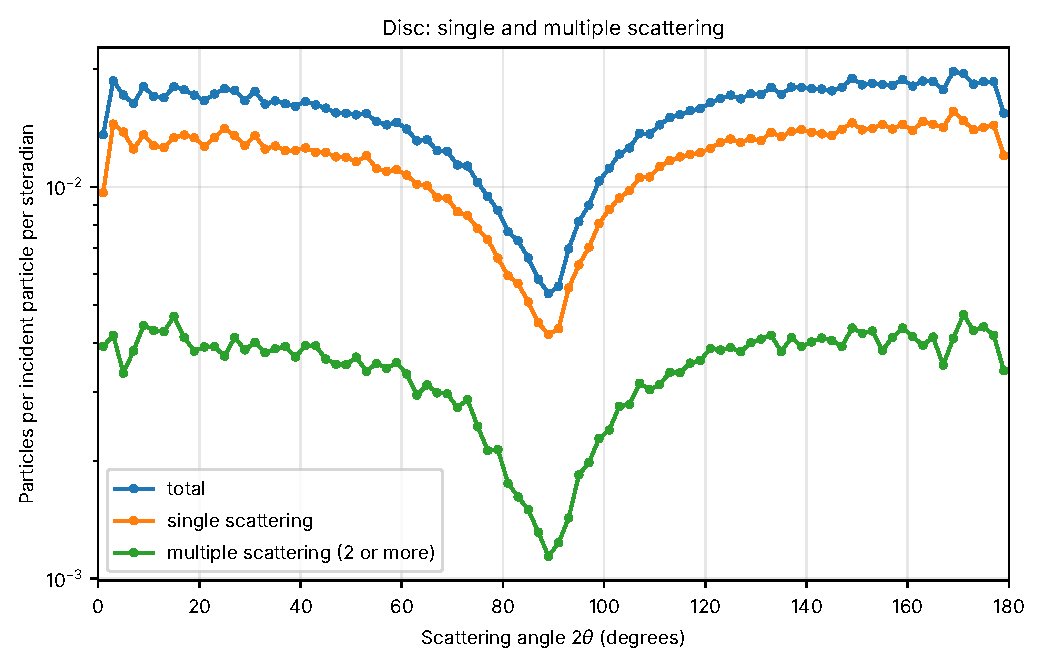
\includegraphics[width=0.78\textwidth]{fig_orders_disc}
  \caption{Example disc perpendicular to the beam: single and multiple scattering per steradian, $10^6$ incident particles.}
  \label{fig:ordersdisc}
\end{figure}

\begin{figure}[H]
  \centering
  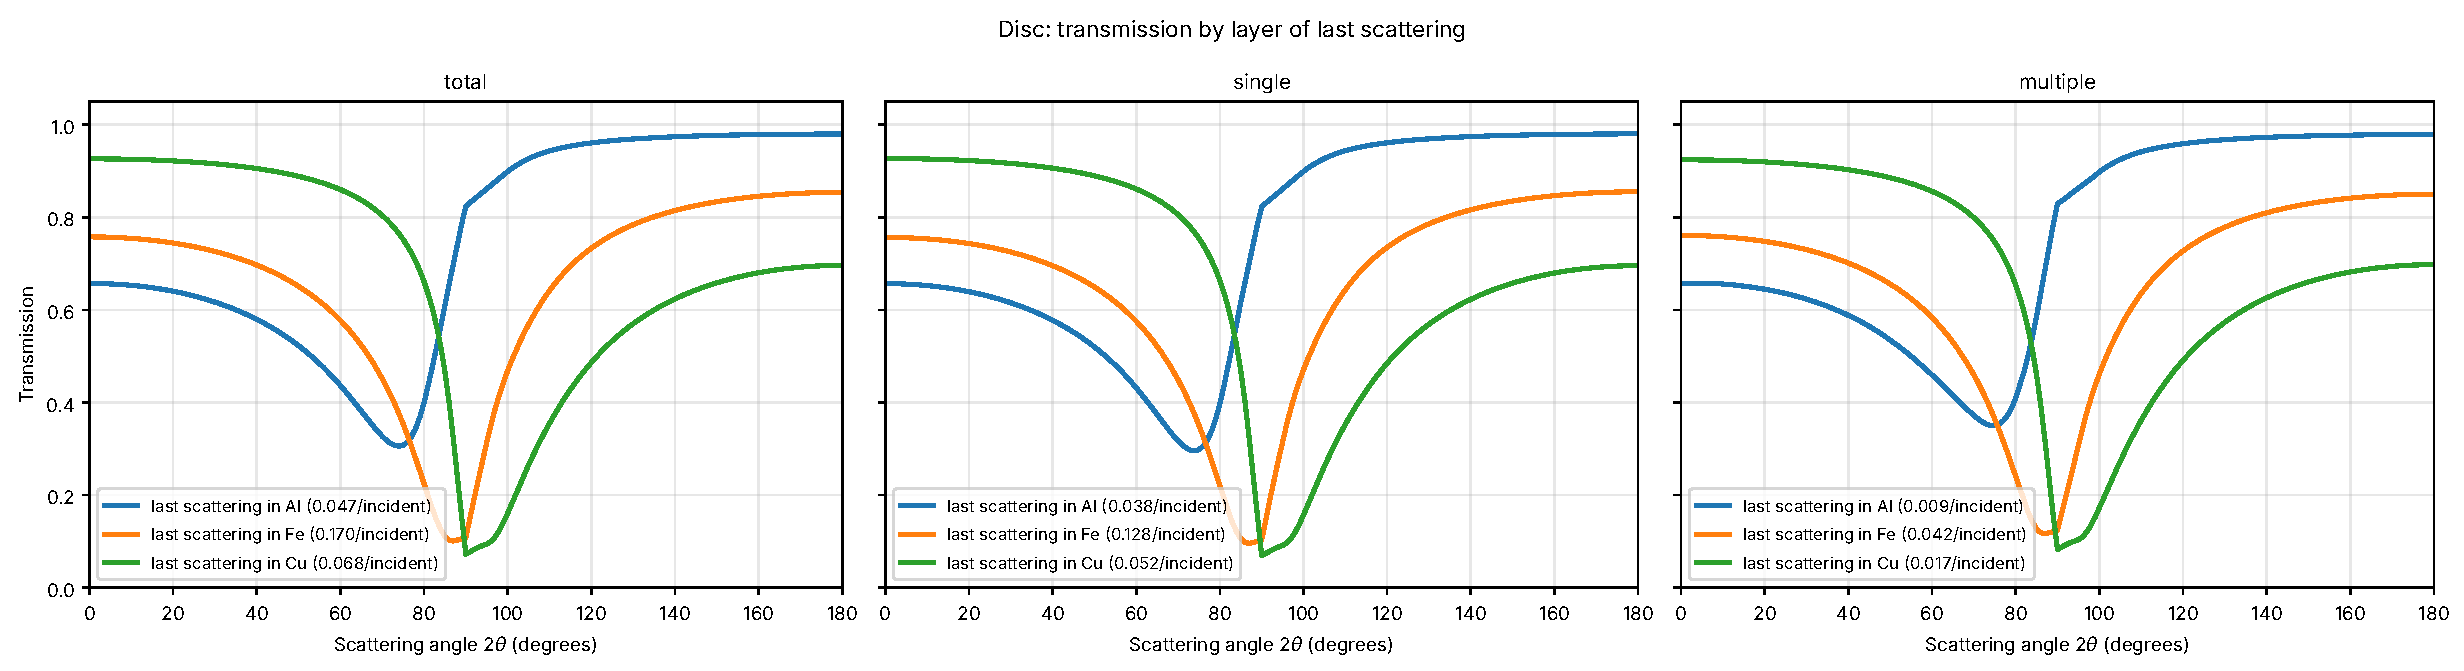
\includegraphics[width=\textwidth]{fig_bylayer_disc}
  \caption{Example disc: transmission by layer of last scattering (Chapter~\ref{ch:lastlayer}).}
  \label{fig:bylayerdisc}
\end{figure}

\paragraph{Disc or square plate?} Figure~\ref{fig:discvsslab} compares the disc with the square slab of side $D$ (the smallest
square that contains it), with the same layers and the same beam.
\begin{itemize}
  \item The transmission is the same at all angles except near $90^\circ$, where the particles leave through the edge. There the
        disc transmits more: at height $y$ its edge is at $\sqrt{R^2-y^2}$ from the axis, closer than the side of the square.
        At $90^\circ$ the transmission is 0.172 (disc) against 0.166 (square) for $D=20$~mm, and 0.430 against 0.382 for
        $D=10$~mm.
  \item The ratio of multiple to single scattering is slightly smaller in the disc, which has less material away from the beam:
        0.214 against 0.230 for $D=9$~mm, 0.299 against 0.303 for $D=20$~mm. The difference vanishes for large discs (0.318 for
        both at $D=40$~mm), where few particles reach the edge.
\end{itemize}

\begin{figure}[H]
  \centering
  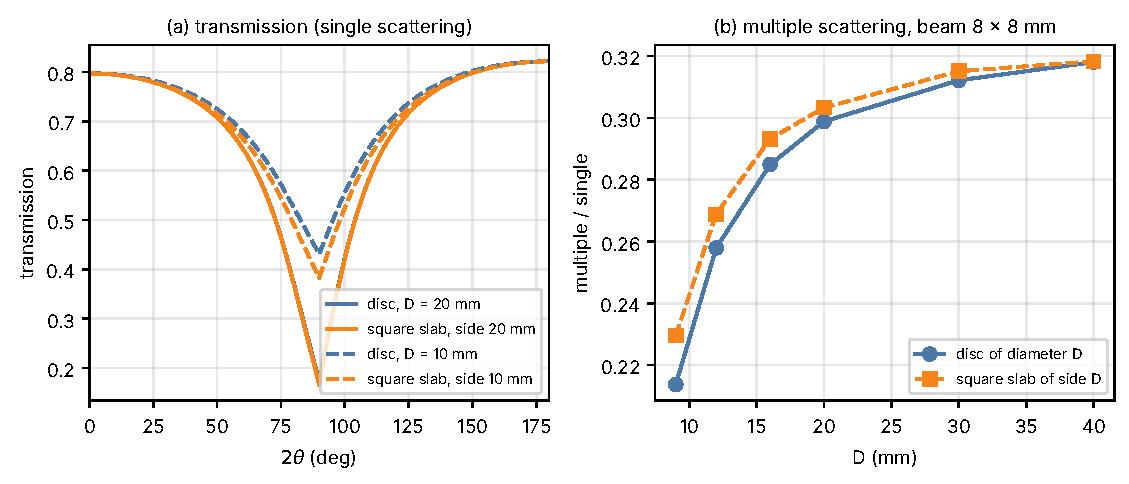
\includegraphics[width=\textwidth]{fig_disc_vs_slab}
  \caption{Disc of diameter $D$ and square slab of side $D$, same layers, normal incidence, beam $8\times8$~mm. (a)~Transmission
  versus $\twotheta$ for $D=20$ and 10~mm. (b)~Ratio of multiple to single scattering versus $D$ ($3\times10^5$ particles per point).}
  \label{fig:discvsslab}
\end{figure}

\paragraph{Validation.} Figure~\ref{fig:discvalid} shows the fraction of a square beam that hits a thin, strongly absorbing disc
(every particle that meets it interacts), for several beam sizes and orientations, against the area of the face seen along the
beam: they agree within the statistical error. The other checks are listed in Chapter~\ref{ch:validation}.

\begin{figure}[H]
  \centering
  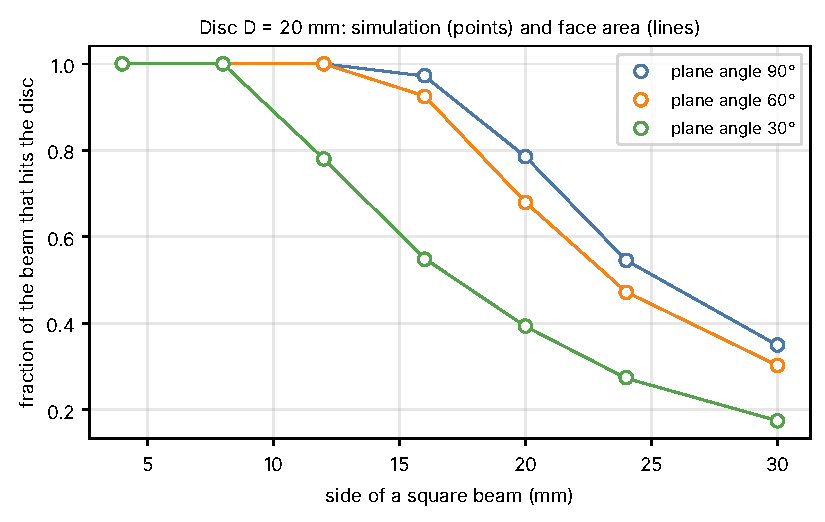
\includegraphics[width=0.78\textwidth]{fig_disc_validation}
  \caption{Disc of 20~mm, 0.01~mm thick, $\mu = 10^4$~mm$^{-1}$: fraction of the beam that interacts (points, $2\times10^5$
  particles each) and \code{face_area_in_beam}$/(w_b h_b)$ (lines), for a square beam of increasing size and three orientations.}
  \label{fig:discvalid}
\end{figure}

\section{With the other modules and the main script}

\begin{itemize}
  \item \code{transmission_vs_angle}, \code{simulate_scattering_orders}, \code{transmission_by_last_layer} and the direct method
        (\code{attenuation_factors_direct}, Chapter~\ref{ch:direct}) accept a disc as they accept a slab or a cylinder.
  \item The main script has the geometry \code{disc}, with the layers \code{DISC_LAYERS} and the diameter \code{DISC_DIAMETER}
        set at the top of \file{run\_simulation.py}; \code{--plane-angle}, \code{--bottom}, \code{--height} and \code{--fullness}
        work as for the slab (Chapter~\ref{ch:main}):
\end{itemize}
\begin{lstlisting}[style=shell]
python run_simulation.py --geometry disc
python run_simulation.py --geometry disc --plane-angle 45
python run_simulation.py --geometry disc --bottom -10 --height 9
\end{lstlisting}

\begin{note}[Discs and \textsc{correct}]
\textsc{correct} (and \textsc{pycorrect}) has no disc geometry: its flat-plate routine \code{PLATE} treats an \emph{infinite} plate.
For a disc larger than the beam this is exact as long as the scattered particles leave through the faces, and it fails near the
grazing directions ($\twotheta\approx 180^\circ-\alpha$ and its mirror), where they leave through the edge. The direct method of
\mcams\ gives the exact factors of the disc at every angle.
\end{note}

\section{Assumptions and limits}

\begin{itemize}
  \item The disc is \textbf{centred on the beam}, horizontally and vertically. An offset disc would need a centre $(x_0, y_0)$ in the
        section test; it is listed among the possible extensions (Chapter~\ref{ch:limits}).
  \item All the layers have the \textbf{same diameter}. A circular cell whose windows are larger than the sample, or a ring that holds
        the sample, needs layers of different diameters (a ring would be a layer with an inner and an outer radius).
  \item The edge of the disc is a plain cylindrical surface: no rim, no clamp, no holder.
\end{itemize}
